\documentclass[spanish,12pt,letterpapper]{article}
\usepackage{babel}
\usepackage[utf8]{inputenc}
\usepackage{graphicx}
\usepackage{hyperref}
\begin{document}
	\begin{titlepage}
		\begin{center}
			
\includegraphics[width=0.6\textwidth]{../logoUnADM}~\\[1cm] 
			\textsc{Universidad Abierta y a Distancia de México}\\[0.8cm]
			\textsc{Desarrollo de Software}\\[1.8cm]
			
			\textbf{ \Large Evidencia de aprendizaje. Diagrama del negocio }\\[3cm]
			
			Diego Antonio Plascencia Lara\\ ES1421004131 \\[0.4cm]
			Facilitador(a): Julia Alicia Reyes Rios\\
			Materia: Modelado de Negocios\\
			Grupo: DS-DMDN-1601-B1-007 \\
			Unidad: III \\
			
			\vfill México D.F\\{\today}
			
		\end{center}
	\end{titlepage}
	
	\section{Instrucciones}	
	Evidencia de aprendizaje: Para desarrollar la evidencia de aprendizaje U2 deberá apoyarse en un diagrama de la unidad anterior.\\
	\paragraph{Dinámica:\\}	
Identificación de los elementos de UML Y BPMN (5 puntos)\\
Coherencia (4 puntos)\\
\paragraph{Actores:\\}
Identificación de los actores en relación directa con el caso (4)\\
Interacción (4).\\
Información que maneja (4)\\
Funciones asignadas (4)\\
\paragraph{Diagrama BPMN:\\} 
Elementos completos (5)\\
Actividades identificadas en relación con el caso (5)\\
Actores identificados en relación con el caso (5)\\
Secuencia lógica y ordenada (5)\\
\paragraph{Diagrama de actividades:\\} 
Elementos completos, inicio y fin, actividades y flujos (5)\\
Actividades identificadas en relación con el caso (5)\\
Secuencia lógica y ordenada (5)\\
\paragraph{Diagramas de casos de uso:\\} 
Elementos completos (5)\\
Actividades identificadas en relación con el caso de uso (5)\\
Actores identificados y diagramados en relación con el caso (5)\\
Total: 100 puntos
	
	\subsection{Requerimientos}
	
	``EL ENTRENAMIENTO AUDITIVO INTERACTIVO''\\
	
	``El entrenamiento auditivo de un músico es una de las tareas más importantes para su vida profesional. En su etapa formativa es uno de los aspectos que deberían considerarse prioritarios, sin embargo, esto no necesariamente ocurre. Es una labor tediosa y difícil de llevar a cabo, especialmente en su etapa inicial. Para cubrir esta necesidad primordial, un grupo de maestros de asignaturas teórico musicales decidió plantear un subproyecto PAPIME para la implementación de un Laboratorio de Entrenamiento Auditivo Interactivo en la Escuela Nacional de Música, en donde los estudiantes pudieran acudir a trabajar de forma individual y utilizar programas computacionales que los ayudaran en su entrenamiento auditivo, mejorando la calidad de su formación musical''
	
	\section{Dinámica}
	\subsection{Actividades}
	Proceso ``Uso del Laboratorio'':\\
	
	\begin{itemize}
	\item Solicitar el Permiso de Uso del Recurso
	\item Usar Software Correspondiente al Objetivo
	\item Terminar la Practica y Abandonar el Aula
	\item Otorgar Recursos
	\item Verificar el correcto uso de los recursos
	\item Registrar Salidas
	\item Dar mantenimiento al equipo de computo
	\item Atender Solicitudes de Reemplazo de Equipo
	\end{itemize}
	
	\section{Actores}
	
		\textbf{ALUMNO:\\}	
	Solicitar el Permiso de Uso del Recurso\\
	Usar Software Correspondiente al Objetivo\\
	Terminar la Practica y Abandonar el Aula\\
	
	\textbf{RECEPCIONISTA:\\}	
	Otorgar Recursos\\
	Verificar el correcto uso de los recursos\\
	Registrar Salidas\\
	Dar mantenimiento al equipo de computo\\

	\textbf{DIRECCIÓN GENERAL DE COMPUTO:\\}
	Atender Solicitudes de Reemplazo de Equipo
	
	\subsection{Conexiones}
	El proceso empieza cuando un alumno requiere utilizar el laboratorio.\\
	Solicitar recurso esta conectada a una compuerta condicional, si se identifica el alumno se procede a la tarea ``Usa el Software'', si no se termina el proceso.\\
	La tarea ``Usa el Software`` tiene una conexión de mensaje a ``Registrar entrada'' en el pool ``Auxiliar técnico'', en este pool hasta la tarea ``Registrar salida'' donde regresa un mensaje al Alumno, también en la actividad ``Dar mantenimiento al equipo hay un mensaje bidireccional con la única actividad (``Atender solicitudes de equipo nuevo'') de DGDC.
	
	Por lo que las conexiones de \textbf{mensaje} son entre:

	\begin{itemize}
	 \item \textbf{``Usar el Software'' (alumno) - ``Registrar entrada'' (aux. tec.)} 
	 \item \textbf{``Registrar salida'' (aux. tec.) - ``Terminar sesion'' (alumno)} y 
	 \item \textbf{``Dar mantenimiento al equipo'' (aux. tec.) - ``Atender solicitudes de equipo nuevo'' (dgdc)}
	\end{itemize}

	
	\section{Diagrama BPMN}
	
	\begin{center}
	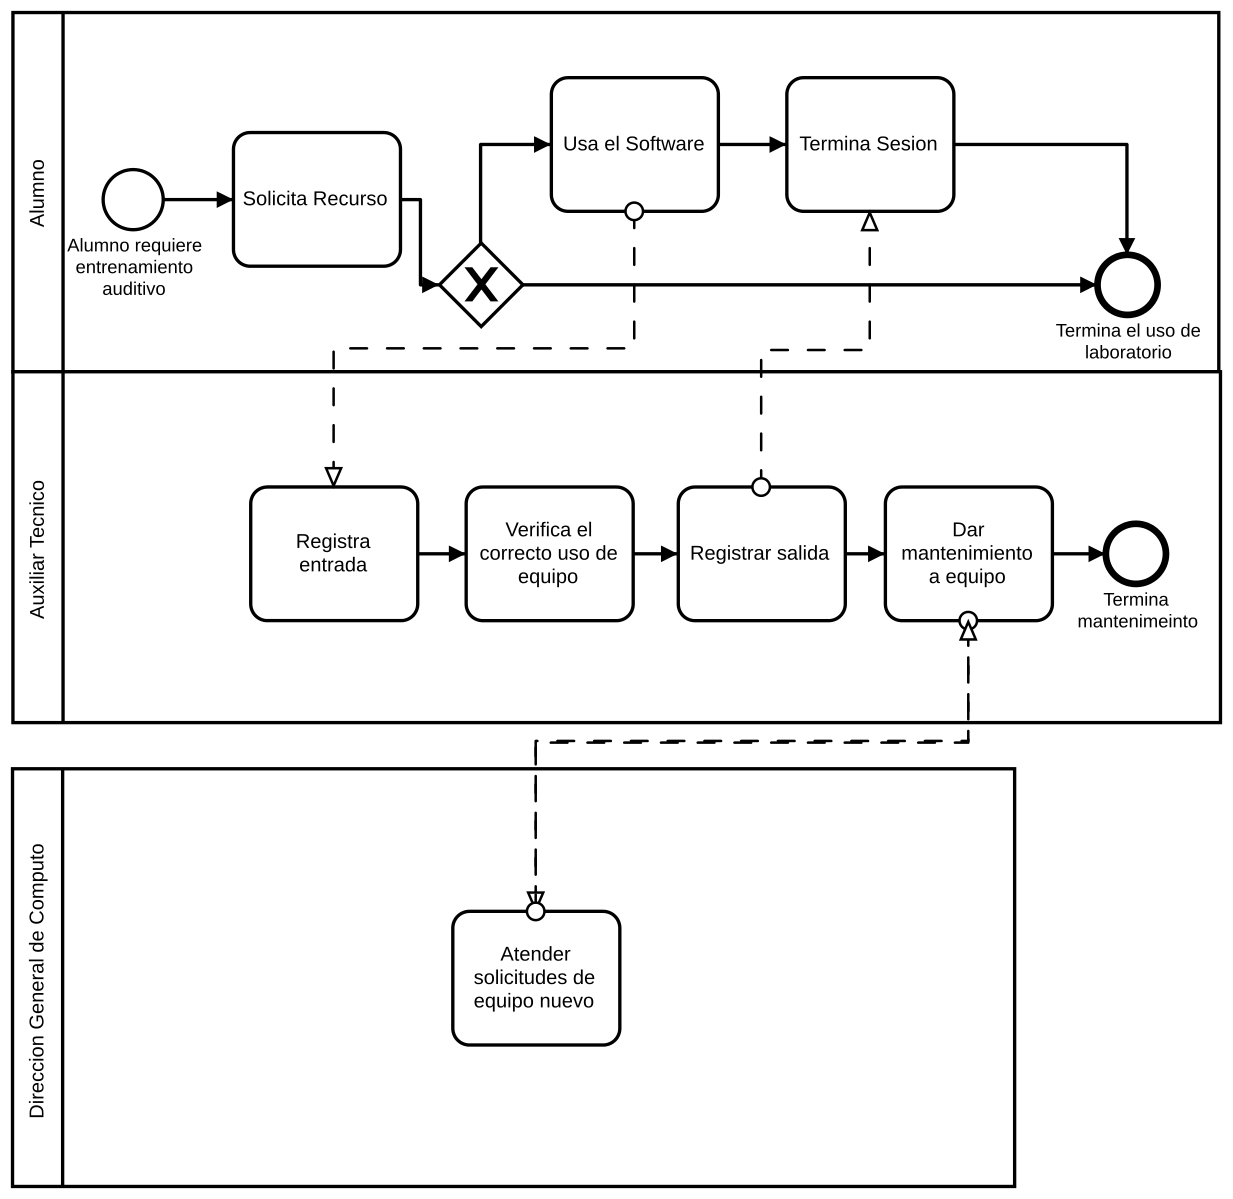
\includegraphics[width=1\textwidth]{./bpmn}~\\[1cm]
	\end{center}
	
	En el diagrama se muestran las tareas principal, divididas por pools que en este caso son las personas o actores (alumno, técnico, la dgdc) que se comunican entre si por medio de vínculos de mensajes. Al final se logra un correcto uso del laboratorio.
	
	
	\section{Diagrama de Actividades}
	\begin{center}
	\includegraphics[width=1\textwidth]{./activities}~\\[1cm]
	\end{center}
	
	Este diagrama UML es similar al de BPMN, pero en este diagrama de actividades se puede observar mas el paralelismo, es decir las actividades que realizan 2 o mas actores al mismo tiempo.
	
	\section{Diagramas de casos de Uso}
	\begin{center}
	\includegraphics[width=1\textwidth]{./usecases}~\\[1cm]
	\end{center}
	
	En el diagrama se observan los 3 actores principales del proceso en la unidad anterior. Las actividades pasan a ser casos de uso y las sub-actividades a casos de uso con relación de inclusión, y las tareas en común extienden de una mas general.
	
	
	
	
	\pagebreak
	\begin{thebibliography}{9}
	\bibitem{maturanaModelamiento} Object Management Group. 
		\emph{Business Process Model and Notation}. {[} Fecha de consulta: \today {]}. Disponible en: \textless http://www.bpmn.org/ \textgreater	
	
		\bibitem{maturanaModelamiento} Maturana Ortiz, Jorge. 
		\emph{Modelamiento de Software y Negocios}. {[} Fecha de consulta: \today {]}. Disponible en: \textless http://www.info.univ-angers.fr/pub/maturana/files/Modelamiento\_de\_Software\_y\_Negocios.pdf \textgreater
		
		\bibitem{panAdm} León León, Oyuky María \& Asato España, Julio Armando. 
		\emph{La Importancia del Modelado de Procesos de
			Negocio como Herramienta para la Mejora e
			Innovación}. Panorama administrativo {[}en linea{]}, México. 2009, vol.4 num. 7  {[} Fecha de consulta: \today {]}. Disponible en: \textless http://132.248.9.34/hevila/Panoramaadministrativo/2009/no7/4.pdf \textgreater
	\end{thebibliography}
\end{document}